% !TeX program = xelatex
\ifdefined\BookMaster\else
\documentclass[11pt,oneside]{article}
% !TeX program = xelatex
\usepackage[b5paper,left=22mm,right=22mm,top=20mm,bottom=22mm,footskip=11mm]{geometry}
\usepackage{fontspec}
\setmainfont{TeX Gyre Termes}
\setsansfont{TeX Gyre Heros}
\usepackage{amsmath,amssymb,mathtools,amsthm}
\renewcommand{\cdots}{\mathinner{\cdotp\cdotp\cdotp}}
\usepackage{graphicx,adjustbox,array,booktabs,longtable,multirow,enumitem,changepage,needspace}
\usepackage[table]{xcolor}
\usepackage{fancyhdr}
\raggedbottom
\interfootnotelinepenalty=10000
\newcommand{\BookFootnote}[2]{\begingroup\renewcommand{\thefootnote}{\fnsymbol{footnote}}\footnote[#1]{#2}\endgroup}
\newcommand{\BookFootnoteMark}[1]{\begingroup\renewcommand{\thefootnote}{\fnsymbol{footnote}}\footnotemark[#1]\endgroup}
\newcommand{\BookFootnoteText}[2]{\begingroup\renewcommand{\thefootnote}{\fnsymbol{footnote}}\footnotetext[#1]{#2}\endgroup}
\newenvironment{BookFloat}[1]{\par\addvspace{.6\baselineskip}\noindent\def\BookFloatID{#1}\begin{minipage}{\linewidth}\phantomsection\label{bookfloat:#1:start}}{\phantomsection\label{bookfloat:\BookFloatID:end}\end{minipage}\par\addvspace{.6\baselineskip}}

\usepackage[unicode,hidelinks]{hyperref}
\pagestyle{fancy}
\fancyhf{}
\newcommand{\BookFooter}{}
\fancyfoot[L]{\parbox[b]{\dimexpr\textwidth-15mm}{\footnotesize\BookFooter}}
\fancyfoot[R]{\footnotesize\thepage}
\renewcommand{\headrulewidth}{0pt}
\renewcommand{\footrulewidth}{0pt}
\setlength{\parindent}{0pt}
\setlength{\parskip}{0.2em}
\setlength{\emergencystretch}{3em}
\setlist{nosep,leftmargin=1.7em,labelsep=.65em}
\newif\ifBookNarrative
\BookNarrativetrue
\newenvironment{BookBody}{\setlength{\parindent}{0pt}}{}
\newcommand{\BookStatement}[1]{\par\addvspace{.6\baselineskip}\noindent #1\enspace\ignorespaces}
\newcommand{\BookLabel}[1]{\par\addvspace{.6\baselineskip}\needspace{3\baselineskip}\noindent\textbf{#1}\quad\ignorespaces}
\newcommand{\BookHeading}[1]{\par\addvspace{\baselineskip}\needspace{4\baselineskip}\noindent{\large\bfseries #1}\par\medskip}
\newcommand{\BookSubheading}[1]{\par\addvspace{.7\baselineskip}\needspace{3\baselineskip}\noindent{\bfseries #1}\par\smallskip}
\newcommand{\BookTextHeading}[1]{\par\addvspace{.7\baselineskip}\needspace{3\baselineskip}\noindent #1\par\smallskip}
\newcommand{\BookSectionTitle}[2]{\par\addvspace{1.2\baselineskip}\needspace{5\baselineskip}\noindent\colorbox{gray!25}{\sffamily\bfseries\small SECTION #1}\quad{\large\bfseries #2}\par\medskip}
\newcommand{\BookExerciseTitle}[1]{\par\addvspace{\baselineskip}\needspace{4\baselineskip}\noindent{\color{gray}\rule{1.5mm}{1.5mm}}\enspace{\large\bfseries Exercises #1}\par\medskip}
\newcommand{\BookBullet}[1]{\begin{list}{\textbullet}{\setlength{\leftmargin}{1.7em}\setlength{\labelwidth}{1em}\setlength{\labelsep}{.7em}\setlength{\topsep}{0pt}\setlength{\parsep}{0pt}\setlength{\itemsep}{0pt}}\item #1\end{list}}
\newcommand{\BookExercise}[2]{\begin{list}{\textbf{#1}}{\setlength{\leftmargin}{2.2em}\setlength{\labelwidth}{1.5em}\setlength{\labelsep}{.7em}\setlength{\topsep}{.15em}\setlength{\parsep}{0pt}\setlength{\itemsep}{0pt}}\item #2\end{list}}
\newcommand{\BookEnd}[1]{\unskip\nobreak\hfill\ensuremath{#1}}
\newcommand{\BookSource}[2]{\phantomsection\label{sourcepage:#1}} % Source-page anchors, retained through reflow.
\usepackage{multicol}
\usepackage{tikz}
\newcommand{\BookPartEntry}[2]{\par\noindent\makebox[17mm][l]{\bfseries Section #1}#2\par}
\newcommand{\BookPartTitle}[3]{\par\bigskip\noindent\begin{tikzpicture}\node[anchor=north west,inner sep=0pt,outer sep=0pt] (bookpart) at (0,0) {\begin{minipage}{\dimexpr\linewidth-.5pt}\hspace*{26mm}\begin{minipage}[t]{\dimexpr\linewidth-26mm}\begin{adjustbox}{max width=\linewidth}{\fontsize{20}{24}\selectfont\bfseries #2}\end{adjustbox}\par\vspace{6mm}\hrule\vspace{6mm}{\sffamily\footnotesize\setlength{\parskip}{.3em}#3}\vspace{3mm}\end{minipage}\end{minipage}};\path[shade,top color=gray!60,bottom color=white] (0,0) rectangle ([xshift=24mm]bookpart.south west);\node[anchor=north,font=\sffamily\bfseries\small] at (12mm,-2mm) {PART};\node[anchor=north,font=\sffamily\bfseries\Huge] at (12mm,-7mm) {#1};\end{tikzpicture}\par\bigskip}
\newsavebox{\BookMathBox}
\makeatletter
\newcommand{\BookInline}[1]{\leavevmode\hskip0pt\relax\begingroup\in@{\begin}{#1}\ifin@\sbox{\BookMathBox}{\(#1\)}\ifdim\wd\BookMathBox>\dimexpr\linewidth-1em\relax\resizebox{\dimexpr\linewidth-1em\relax}{!}{\usebox{\BookMathBox}}\else\(#1\)\fi\else\in@{\left}{#1}\ifin@\sbox{\BookMathBox}{\(#1\)}\ifdim\wd\BookMathBox>\dimexpr\linewidth-1em\relax\resizebox{\dimexpr\linewidth-1em\relax}{!}{\usebox{\BookMathBox}}\else\(#1\)\fi\else\(#1\)\fi\fi\endgroup\hskip0pt\relax}
\makeatother
\DeclareMathOperator{\Aut}{Aut}
\DeclareMathOperator{\End}{End}
\DeclareMathOperator{\Hom}{Hom}
\DeclareMathOperator{\GF}{GF}
\DeclareMathOperator{\irr}{irr}
\DeclareMathOperator{\lt}{lt}
\DeclareMathOperator{\lp}{lp}
\providecommand{\textcircled}[1]{\textnormal{(#1)}}

\begin{document}
\fi
\renewcommand{\BookFooter}{Section 23 Integral Domains}
\pdfbookmark[0]{Section 23 Integral Domains}{23_integral_domains}
\ifdefined\BookMaster\else\setcounter{page}{194}\fi
% Source PDF page 211; original printed page 194
\BookSource{211}{194}
\BookNarrativetrue

\begin{BookBody}

\BookSectionTitle{23}{Integral Domains}

\noindent While a careful treatment of polynomials is not given until Section 27, for purposes of motivation we shall make intuitive use of them in this section.

\BookTextHeading{\textbf{Divisors of Zero and Cancellation}  }

\noindent One of the most important algebraic properties of our usual number system is that a product of two numbers can be 0 only if at least one of the factors is 0. We have used this fact many times in solving equations, perhaps without realizing that we were using it. Suppose, for example, we are asked to solve the equation

\begin{center}\begin{adjustbox}{max width=\linewidth}\BookInline{\displaystyle x^{2}- 5x+ 6= 0.}\end{adjustbox}\end{center}

\noindent The first thing we do is factor the left side:

\begin{center}\begin{adjustbox}{max width=\linewidth}\BookInline{\displaystyle x^{2}- 5x+ 6= (x- 2)(x- 3).}\end{adjustbox}\end{center}

\noindent Then we conclude that the only possible values for \BookInline{x} are 2 and 3. Why? The reason is that if \BookInline{x} is replaced by any number \BookInline{a,\allowbreak } the product \BookInline{(a- 2)(a- 3)} of the resulting numbers is 0 if and only if either \BookInline{a- 2= 0} or \BookInline{a- 3= 0.}

\BookLabel{23.1 Example} Solve the equation \BookInline{x^{2}- 5x+ 6= 0} in \BookInline{\mathbb{Z}_{12}.}

\BookLabel{\textit{Solution}} The factorization \BookInline{x^{2}- 5x+ 6= (x- 2)(x- 3)} is still valid if we think of \BookInline{x} as standing for any number in \BookInline{\mathbb{Z}_{12}.} But in \BookInline{\mathbb{Z}_{12},\allowbreak } not only is \BookInline{0a= a0= 0} for all \BookInline{a\in \mathbb{Z}_{12},\allowbreak } but also

\begin{center}\begin{adjustbox}{max width=\linewidth}\BookInline{\displaystyle \begin{aligned}(2)(6)&= (6)(2)= (3)(4)= (4)(3)= (3)(8)= (8)(3) \\ &= (4)(6)= (6)(4)= (4)(9)= (9)(4)= (6)(6)= (6)(8) \\ &= (8)(6)= (6)(10)= (10)(6)= (8)(9)= (9)(8)= 0.\end{aligned}}\end{adjustbox}\end{center}

\noindent We find, in fact, that our equation has not only 2 and 3 as solutions, but also 6 and 11, for \BookInline{(6- 2)(6- 3)= (4)(3)= 0} and \BookInline{(11- 2)(11- 3)= (9)(8)= 0} in \BookInline{\mathbb{Z}_{12}.}\BookEnd{\blacktriangle}

These ideas are of such importance that we formalize them in a definition.

\BookLabel{23.2 Definition} If \BookInline{a} and \BookInline{b} are two nonzero elements of a ring \BookInline{R} such that \BookInline{ab= 0,\allowbreak } then \BookInline{a} and \BookInline{b} are \textbf{divisors of 0} (or\textbf{ 0 divisors}\BookInline{).}\BookEnd{\blacksquare}

\end{BookBody}

% Source PDF page 212; original printed page 195
\BookSource{212}{195}
\BookNarrativetrue

\begin{BookBody}

Example 23.1 shows that in \BookInline{\mathbb{Z}_{12}} the elements 2, 3, 4, 6, 8, 9, and 10 are divisors of 0. Note that these are exactly the numbers in \BookInline{\mathbb{Z}_{12}} that are not relatively prime to 12, that is, whose gcd with 12 is not 1.

If \BookInline{R} is a ring with unity and \BookInline{a} is a unit in \BookInline{R,\allowbreak } then \BookInline{a} is not a divisor of 0. To see this, note that if \BookInline{ab= 0,\allowbreak } then \BookInline{a^{- 1}ab= 0,\allowbreak } so \BookInline{b= 0.} Similarly, if \BookInline{ba= 0,\allowbreak } then \BookInline{baa^{- 1}= 0,\allowbreak } so \BookInline{b= 0.} Theorem 23.3 shows that in the ring \BookInline{\mathbb{Z}_{n}} every element is either 0, a unit, or a 0 divisor.

\BookLabel{23.3 Theorem} Let \BookInline{m\in \mathbb{Z}_{n}.} Either \BookInline{m= 0,\allowbreak m} is relatively prime to \BookInline{n,\allowbreak } in which case \BookInline{m} is a unit in \BookInline{\mathbb{Z}_{n},\allowbreak } or \BookInline{m} is not relatively prime to \BookInline{n,\allowbreak } in which case \BookInline{m} is a 0 divisor in \BookInline{\mathbb{Z}_{n}.}

\BookLabel{\textit{Proof}} We first suppose that \BookInline{m\neq 0} and gcd\BookInline{(m,\allowbreak n)= d\neq 1.} Then, using integer multiplication

\begin{center}\begin{adjustbox}{max width=\linewidth}\BookInline{\displaystyle m \left( \frac{n}{d} \right) = \left( \frac{m}{d} \right) n}\end{adjustbox}\end{center}

\noindent is a multiple of \BookInline{n,\allowbreak } so in \BookInline{\mathbb{Z}_{n},\allowbreak }

\begin{center}\begin{adjustbox}{max width=\linewidth}\BookInline{\displaystyle m \left( \frac{n}{d} \right) = 0 \in \mathbb{Z}_n.}\end{adjustbox}\end{center}

\noindent Neither \BookInline{m} nor \BookInline{n/d} is 0 in \BookInline{\mathbb{Z}_{n}.} Thus \BookInline{m} is a divisor of 0.

Now suppose that gcd\BookInline{(m,\allowbreak n)= 1.} Then there are integers \BookInline{a} and \BookInline{b} such that \textit{an} \BookInline{+ bm= 1.} By the division algorithm, there are integers \BookInline{q} and \BookInline{r} such that \BookInline{0\leq } \BookInline{r\leq n- 1} and \BookInline{b= nq+ r.} We can write

\begin{center}\begin{adjustbox}{max width=\linewidth}\BookInline{\displaystyle rm= (b- nq)m= bm- nqm= (1- an)- nqm= 1- n(a+ qm).}\end{adjustbox}\end{center}

\noindent So in \BookInline{\mathbb{Z}_{n},\allowbreak rm= mr= 1} and \BookInline{m} is a unit. \BookEnd{\blacklozenge}

\BookLabel{23.4 Example} Classify each nonzero element of \BookInline{\mathbb{Z}_{20}} as a unit or a 0 divisor.

\BookLabel{\textit{Solution}} The greatest common divisor of \BookInline{m} and 20 is 1 if \BookInline{m= 1,\allowbreak 3,\allowbreak 7,\allowbreak 9,\allowbreak 11,\allowbreak 13,\allowbreak 17,\allowbreak 19,\allowbreak } so these are all units. For \BookInline{m= 2,\allowbreak 4,\allowbreak 5,\allowbreak 6,\allowbreak 8,\allowbreak 10,\allowbreak 12,\allowbreak 14,\allowbreak 15,\allowbreak 16,\allowbreak 18,\allowbreak } gcd\BookInline{(m,\allowbreak 20)>1,\allowbreak } so these are all 0 divisors. We see that

\begin{center}\begin{adjustbox}{max width=\linewidth}\BookInline{\displaystyle 1\cdot 1= 3\cdot 7= 9\cdot 9= 11\cdot 11= 13\cdot 17= 19\cdot 19= 1\in \mathbb{Z}_{20}}\end{adjustbox}\end{center}

\noindent which verifies that each is a unit. We also see that

\begin{center}\begin{adjustbox}{max width=\linewidth}\BookInline{\displaystyle 2\cdot 10= 4\cdot 5= 6\cdot 10= 8\cdot 15= 12\cdot 5= 14\cdot 10= 16\cdot 5= 18\cdot 10= 0\in \mathbb{Z}_{20}}\end{adjustbox}\end{center}

\noindent which verifies that each of these is a 0 divisor in \BookInline{\mathbb{Z}_{20}.} \BookEnd{\blacktriangle}

\BookLabel{23.5 Corollary} If \BookInline{p} is a prime number, then every nonzero element of \BookInline{\mathbb{Z}_{p}} is a unit, which means that \BookInline{\mathbb{Z}_{p}} is a field and it has no divisors of 0.

\BookLabel{\textit{Proof}} For any \BookInline{0<m\leq p- 1,\allowbreak } gcd\BookInline{(m,\allowbreak p)= 1.} So \BookInline{m} is a unit in \BookInline{\mathbb{Z}_{p}} by Theorem 23.3. \BookEnd{\blacklozenge}

The preceding corollary shows that when we consider the ring \BookInline{M_{n}(\mathbb{Z}_{p}),\allowbreak } we are talking about a ring of matrices over a \BookInline{\text{fi}eld.} In the typical undergraduate linear algebra course, only the field properties of the real or complex numbers are used in much of the work. Such notions as matrix reduction to solve linear systems, determinants, Cramer’s rule, eigenvalues and eigenvectors, and similarity transformations to try to diagonalize a matrix are valid using matrices over any field; they depend only on the arithmetic properties of a field. Considerations of linear algebra involving notions of magnitude, such 
% Source PDF page 213; original printed page 196
\BookSource{213}{196}
as least-squares approximate solutions or orthonormal bases, make sense only when using fields where we have an idea of magnitude. The relation

\end{BookBody}

\BookNarrativetrue

\begin{BookBody}

\begin{center}\begin{adjustbox}{max width=\linewidth}\BookInline{\displaystyle p\cdot 1= 1+ 1+ \cdots + 1= 0}\end{adjustbox}\end{center}

\BookInline{p} summands

\noindent indicates that there can be no very natural notion of magnitude in the field \BookInline{\mathbb{Z}_{p}.}

Another indication of the importance of the concept of 0 divisors is shown in the following theorem. Let \BookInline{R} be a ring, and let \BookInline{a,\allowbreak b,\allowbreak c\in R.} The\textbf{ cancellation laws} hold in \BookInline{R} if \BookInline{ab= } \textit{ac} with \BookInline{a\neq 0} implies \BookInline{b= c,\allowbreak } and \BookInline{ba= ca} with \BookInline{a\neq 0} implies \BookInline{b= c.} These are multiplicative cancellation laws. Of course, the additive cancellation laws hold in \BookInline{R,\allowbreak } since \BookInline{\langle R,\allowbreak + \rangle } is a group.

\BookLabel{23.6 Theorem} The cancellation laws hold in a ring \BookInline{R} if and only if \BookInline{R} has no divisors of 0.

\BookLabel{\textit{Proof}} Let \BookInline{R} be a ring in which the cancellation laws hold, and suppose \BookInline{ab= 0} for some \BookInline{a,\allowbreak b\in R.} We must show that either \BookInline{a} or \BookInline{b} is 0. If \BookInline{a\neq 0,\allowbreak } then \BookInline{ab= a0} implies that \BookInline{b= 0} by cancellation laws. Therefore, either \BookInline{a= 0} or \BookInline{b= 0.}

Conversely, suppose that \BookInline{R} has no divisors of 0, and suppose that \BookInline{ab= } \textit{ac} with \BookInline{a\neq 0.} Then

\begin{center}\begin{adjustbox}{max width=\linewidth}\BookInline{\displaystyle ab- ac= a(b- c)= 0.}\end{adjustbox}\end{center}

Since \BookInline{a\neq 0,\allowbreak } and since \BookInline{R} has no divisors of 0, we must have \BookInline{b- c= 0,\allowbreak } so \BookInline{b= c.} A similar argument shows that \BookInline{ba= ca} with \BookInline{a\neq 0} implies \BookInline{b= c.}\BookEnd{\blacklozenge}

Suppose that \BookInline{R} is a ring with no divisors of 0. Then an equation\textit{ ax} \BookInline{= b,\allowbreak } with \BookInline{a\neq 0,\allowbreak } in \BookInline{R} can have at most one solution \BookInline{x} in \BookInline{R,\allowbreak } for if \BookInline{ax_{1}= b} and \BookInline{ax_{2}= b,\allowbreak } then \BookInline{ax_{1}= ax_{2},\allowbreak } and by Theorem \BookInline{23.6x_{1}= x_{2},\allowbreak } since \BookInline{R} has no divisors of 0. If \BookInline{R} has unity \BookInline{1\neq 0} and \BookInline{a} is a unit in \BookInline{R} with multiplicative inverse \BookInline{a^{- 1},\allowbreak } then the solution \BookInline{x} of\textit{ ax} \BookInline{= b} is \BookInline{a^{- 1}b.} In the case that \BookInline{R} is commutative, in particular if \BookInline{R} is a field, it is customary to denote \BookInline{a^{- 1}b} and \BookInline{ba^{- 1}(}they are equal by commutativity) by the formal quotient \BookInline{b/a.} This quotient notation must not be used in the event that \BookInline{R} is not commutative, for then we do not know whether \BookInline{b/a} denotes \BookInline{a^{- 1}b} or \BookInline{ba^{- 1}.} In particular, the multiplicative inverse \BookInline{a^{- 1}} of a nonzero element \BookInline{a} of a field may be written \BookInline{1/a.}

\BookTextHeading{\textbf{Integral Domains}  }

\noindent The integers are really our most familiar number system. In terms of the algebraic properties we are discussing\BookInline{,\allowbreak \mathbb{Z}} is a commutative ring with unity and no divisors of 0. Surely this is responsible for the name that the next definition gives to such a structure.

\BookLabel{23.7 Definition} An\textbf{ integral domain} \BookInline{D} is a commutative ring with unity \BookInline{1\neq 0} that contains no divisors of \BookInline{0.}\BookEnd{\blacksquare}

\textit{Thus, if the coefficients of} \BookInline{a} \textit{polynomial are from an integral domain, one can solve} \BookInline{a} \textit{polynomial equation in which the polynomial can be factored into linear factors in} \textit{the usual fashion by setting each factor equal to 0}.

In our hierarchy of algebraic structures, an integral domain belongs between a commutative ring with unity and a field, as we shall show. Theorem 23.6 shows that the cancellation laws for multiplication hold in an integral domain.

\BookLabel{23.8 Example} We have seen that \BookInline{\mathbb{Z}} and \BookInline{\mathbb{Z}_{p}} for any prime \BookInline{p} are integral domains, but \BookInline{\mathbb{Z}_{n}} is not an integral domain if \BookInline{n} is not prime. A moment of thought shows that the direct product \BookInline{R\times S} of two nonzero rings \BookInline{R} and \BookInline{S} is not an integral domain. Just observe that for \BookInline{r\in R} and \BookInline{s\in S} both nonzero, we have \BookInline{(r,\allowbreak 0)(0,\allowbreak s)= (0,\allowbreak 0).}\BookEnd{\blacktriangle}

\end{BookBody}

% Source PDF page 214; original printed page 197
\BookSource{214}{197}
\BookNarrativetrue

\begin{BookBody}

\BookLabel{23.9 Example} Show that although \BookInline{\mathbb{Z}_{2}} is an integral domain, the matrix ring \BookInline{M_{2}(\mathbb{Z}_{2})} has divisors of zero.

\BookLabel{\textit{Solution}} We need only observe that

\begin{center}\begin{adjustbox}{max width=\linewidth}\BookInline{\displaystyle { \binom { 1 \quad 0 } { 0 \quad 0 } } { \binom { 0 \quad 0 } { 1 \quad 0 } } = { \binom { 0 \quad 0 } { 0 \quad 0 } } .}\end{adjustbox}\end{center} \BookEnd{\blacktriangle}

In a field, every nonzero element is a unit. We saw that units cannot be divisors of 0, so in a field there are no divisors of 0. Since multiplication in a field is commutative, every field is an integral domain.

Figure 23.10 gives a Venn diagram view of containment for the algebraic structures having two binary operations with which we will be chiefly concerned. In Exercise 26 we ask you to redraw this figure to include strictly skew fields as well.

We have seen that \BookInline{\mathbb{Q},\allowbreak \mathbb{R},\allowbreak \mathbb{C},\allowbreak } and \BookInline{\mathbb{Z}_{p}} for \BookInline{p} a prime number are all fields. Theorem 23.3 implies that if \BookInline{\mathbb{Z}_{n}} is an integral domain, then \BookInline{\mathbb{Z}_{n}} is a field. In fact, the next theorem says that any finite integral domain is a field. The proof of this theorem is a personal favorite of both authors. It is done by counting, one of the most powerful techniques in mathematics.

\begin{BookFloat}{23_integral_domains-p214-7}
\begin{center}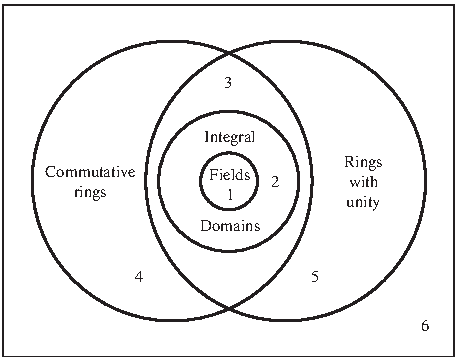
\includegraphics[width=0.626\linewidth,height=.8\textheight,keepaspectratio]{assets/p214_08.pdf}\end{center}
\begin{center}\small\textbf{23.10 Figure}\end{center}
\end{BookFloat}

A collection of rings.

\BookLabel{23.11 Theorem} Every finite integral domain is a field.

\BookLabel{\textit{Proof}} Let \BookInline{R} be a finite integral domain and \BookInline{a} a nonzero element of \BookInline{R.} We wish to show there is an element \BookInline{b\in R} such that \BookInline{ab= 1.} To this end, we define a function \BookInline{f:R\to R} by

\begin{center}\begin{adjustbox}{max width=\linewidth}\BookInline{\displaystyle f(x)= ax.}\end{adjustbox}\end{center}

\noindent We first show that \BookInline{f} is a one-to-one function. Suppose that \BookInline{f(x_{1})= f(x_{2}),\allowbreak } then

\begin{center}\begin{adjustbox}{max width=\linewidth}\BookInline{\displaystyle ax_{1}= ax_{2}}\end{adjustbox}\end{center}

\begin{center}\begin{adjustbox}{max width=\linewidth}\BookInline{\displaystyle x_{1}= x_{2}}\end{adjustbox}\end{center}

\noindent since \BookInline{a\neq 0} and cancellation holds in an integral domain. Thus \BookInline{f} is one-to-one. Since \BookInline{R} is finite and \BookInline{f:R\to R} is one-to-one\BookInline{,\allowbreak f} must also map onto \BookInline{R.} Therefore, there is a \BookInline{b\in R} such that

\begin{center}\begin{adjustbox}{max width=\linewidth}\BookInline{\displaystyle 1= f(a)= ab= ba}\end{adjustbox}\end{center}

\noindent which verifies that \BookInline{a} is a unit. \BookEnd{\blacklozenge}

\end{BookBody}

% Source PDF page 215; original printed page 198
\BookSource{215}{198}
\BookNarrativetrue

\begin{BookBody}

The finite condition in Theorem 23.11 is necessary since \BookInline{\mathbb{Z}} is an infinite integral domain, which is not a field. The counting argument fails in the case where the integral domain is infinite since there are one-to-one functions from an infinite set to itself that are not onto. For example, multiplication by 2 is a one-to-one function mapping \BookInline{\mathbb{Z}} to \BookInline{\mathbb{Z},\allowbreak } but 1 is not in the range of the function.

In Section 39 we will see that other than \BookInline{\mathbb{Z}_{p}} there are many finite integral domains and therefore fields.

\BookTextHeading{\textbf{The Characteristic of a Ring}  }

\noindent Let \BookInline{R} be any ring. We might ask whether there is a positive integer \BookInline{n} such that \BookInline{n\cdot a= 0} for all \BookInline{a\in R,\allowbreak } where \BookInline{n\cdot a} means \BookInline{a+ a+ \cdots + a} for \BookInline{n} summands, as explained in Section 22. For example, the integer \BookInline{m} has this property for the ring \BookInline{\mathbb{Z}_{m}.}

\BookLabel{23.12 Definition} If for a ring \BookInline{R} a positive integer \BookInline{n} exists such that \BookInline{n\cdot a= 0} for all \BookInline{a\in R,\allowbreak } then the least such positive integer is the\textbf{ characteristic of the ring} \BookInline{R.} If no such positive integer exists, then \BookInline{R} is of\textbf{ characteristic} \BookInline{0.}\BookEnd{\blacksquare}

We shall use the concept of a characteristic chiefly for fields. Exercise 35 asks us to show that the characteristic of an integral domain is either 0 or a prime \BookInline{p.}

\BookLabel{23.13 Example} The ring \BookInline{\mathbb{Z}_{n}} is of characteristic \BookInline{n,\allowbreak } while \BookInline{\mathbb{Z},\allowbreak \mathbb{Q},\allowbreak \mathbb{R},\allowbreak } and \BookInline{\mathbb{C}} all have characteristic \BookInline{0.}\BookEnd{\blacktriangle}

At first glance, determination of the characteristic of a ring seems to be a tough job, unless the ring is obviously of characteristic 0. Do we have to examine\textit{ every} element \BookInline{a} of the ring in accordance with Definition 23.12? Our final theorem of this section shows that if the ring has unity, it suffices to examine only \BookInline{a= 1.}

\BookLabel{23.14 Theorem} Let \BookInline{R} be a ring with unity. If \BookInline{n\cdot 1\neq 0} for all \BookInline{n\in \mathbb{Z}^{+ },\allowbreak } then \BookInline{R} has characteristic 0. If \BookInline{n\cdot 1= 0} for some \BookInline{n\in \mathbb{Z}^{+ },\allowbreak } then the smallest such integer \BookInline{n} is the characteristic of \BookInline{R.}

\BookLabel{\textit{Proof}} If \BookInline{n\cdot 1\neq 0} for all \BookInline{n\in \mathbb{Z}^{+ },\allowbreak } then surely we cannot have \BookInline{n\cdot a= 0} for all \BookInline{a\in R} for some positive integer \BookInline{n,\allowbreak } so by Definition \BookInline{23.12,\allowbreak R} has characteristic 0.

Suppose that \BookInline{n} is a positive integer such that \BookInline{n\cdot 1= 0.} Then for any \BookInline{a\in R,\allowbreak } we have

\begin{center}\begin{adjustbox}{max width=\linewidth}\BookInline{\displaystyle n\cdot a= a+ a+ \cdots + a= a(1+ 1+ \cdots + 1)= a(n\cdot 1)= a0= 0.}\end{adjustbox}\end{center}

\noindent Our theorem follows directly. \BookEnd{\blacklozenge}

\end{BookBody}

\BookNarrativefalse

\begin{BookBody}

\BookExerciseTitle{23} \BookEnd{\blacksquare}

\BookTextHeading{\textbf{Computations}}

\BookExercise{1.}{Find all solutions of the equation \BookInline{x^{3}- 2x^{2}- 3x= 0} in \BookInline{\mathbb{Z}_{12}.}}

\BookExercise{2.}{Solve the equation \BookInline{3x= 2} in the field \BookInline{\mathbb{Z}_{7};} in the field \BookInline{\mathbb{Z}_{23}.}}

\BookExercise{3.}{Find all solutions of the equation \BookInline{x^{2}+ 2x+ 2= 0} in \BookInline{\mathbb{Z}_{6}.}}

\BookExercise{4.}{Find all solutions of \BookInline{x^{2}+ 2x+ 4= 0} in \BookInline{\mathbb{Z}_{6}.}}

\noindent In Exercises 5 through 10, find the characteristic of the given ring.

\BookExercise{5.}{\BookInline{2\mathbb{Z}}}

\BookExercise{6.}{\BookInline{\mathbb{Z}\times \mathbb{Z}}}

\BookExercise{7.}{\BookInline{\mathbb{Z}_{3}\times 3\mathbb{Z}}}

\BookExercise{8.}{\BookInline{\mathbb{Z}_{3}\times \mathbb{Z}_{3}}}

\BookExercise{9.}{\BookInline{\mathbb{Z}_{3}\times \mathbb{Z}_{4}}}

\BookExercise{10.}{\BookInline{\mathbb{Z}_{6}\times \mathbb{Z}_{15}}}

\end{BookBody}

% Source PDF page 216; original printed page 199
\BookSource{216}{199}
\BookNarrativefalse

\begin{BookBody}

\noindent In Exercises 11 through 16, classify each nonzero element of the ring as a unit, a divisor of 0, or neither.

\BookExercise{11.}{\BookInline{\mathbb{Z}_{6}}}

\BookExercise{12.}{\BookInline{\mathbb{Z}_{8}}}

\BookExercise{13.}{\BookInline{\mathbb{Z}_{15}}}

\BookExercise{14.}{\BookInline{\mathbb{Z}}}

\BookExercise{15.}{\BookInline{\mathbb{Z}_{3}\times \mathbb{Z}_{3}}}

\BookExercise{16.}{\BookInline{\mathbb{Z}_{4}\times \mathbb{Z}_{5}}}

\BookExercise{17.}{Let \BookInline{R} be a commutative ring with unity of characteristic 4. Compute and simplify \BookInline{(a+ b)^{4}} for \BookInline{a,\allowbreak b\in R.}}

\BookExercise{18.}{Let \BookInline{R} be a commutative ring with unity of characteristic 3. Compute and simplify \BookInline{(a+ b)^{9}} for \BookInline{a,\allowbreak b\in R.}}

\BookExercise{19.}{Let \BookInline{R} be a commutative ring with unity of characteristic 3. Compute and simplify \BookInline{(a+ b)^{6}} for \BookInline{a,\allowbreak b\in R.}}

\BookInline{\Big[\Big]}

\BookExercise{20.}{Show that the matrix \BookInline{\begin{bmatrix} 1 & 2 \\ 2 & 4 \end{bmatrix}} is a divisor of zero in \BookInline{M_{2}(\mathbb{Z}).}}

\BookTextHeading{\textbf{Concepts}}

\noindent In Exercises 21 and 22, correct the definition of the italicized term without reference to the text, if correction is needed, so that it is in a form acceptable for publication.

\BookExercise{21.}{If \BookInline{ab= 0,\allowbreak } then \BookInline{a} and \BookInline{b} are\textit{ divisors of zero}.}

\BookExercise{22.}{If \BookInline{n\cdot a= 0} for all elements \BookInline{a} in a ring \BookInline{R,\allowbreak } then \BookInline{n} is the\textit{ characteristic of} \BookInline{R.}}

\BookExercise{23.}{Determine whether each of the following is true or false.}

\BookExercise{a.}{\textbf{a}\BookInline{.n\mathbb{Z}} has zero divisors if \BookInline{n} is not prime.}

\BookExercise{b.}{Every field is an integral domain.}

\BookExercise{c.}{The characteristic of \BookInline{n\mathbb{Z}} is \BookInline{n.}}

\BookExercise{d.}{As a ring\BookInline{,\allowbreak \mathbb{Z}} is isomorphic to \BookInline{n\mathbb{Z}} for all \BookInline{n\geq 1.}}

\BookExercise{e.}{The cancellation law holds in any ring that is isomorphic to an integral domain.}

\BookExercise{f.}{Every integral domain of characteristic 0 is infinite.}

\BookExercise{g.}{The direct product of two integral domains is again an integral domain.}

\BookExercise{h.}{A divisor of zero in a commutative ring with unity can have no multiplicative inverse.}

\BookExercise{i.}{\textbf{i}\BookInline{.n\mathbb{Z}} is a subdomain of \BookInline{\mathbb{Z}.}}

\BookExercise{j.}{\textbf{j}\BookInline{.\mathbb{Z}} is a subfield of \BookInline{\mathbb{Q}.}}

\BookExercise{24.}{Each of the six numbered regions in Fig. 23.10 corresponds to a certain type of a ring. Give an example of a ring in each of the six cells. For example, a ring in the region numbered 3 must be commutative (it is inside the commutative circle), have unity, but not be an integral domain.}

\BookExercise{25.}{(For students who have had a semester of linear algebra) Let \BookInline{F} be a field. Give five different characterizations of the elements \BookInline{A} of \BookInline{M_{n}(F)} that are divisors of 0.}

\BookExercise{26.}{Redraw Fig. 23.10 to include a subset corresponding to strictly skew fields.}

\BookLabel{\textit{Proof}} \textbf{ Synopsis}

\BookExercise{27.}{Give a one-sentence synopsis of the proof of the “if” part of Theorem 23.6.}

\BookExercise{28.}{Give a two-sentence synopsis of the proof of Theorem 23.11.}

\BookTextHeading{\textbf{Theory}}

\BookExercise{29.}{An element \BookInline{a} of a ring \BookInline{R} is\textbf{ idempotent} if \BookInline{a^{2}= a.} Show that a division ring contains exactly two idempotent elements.}

\BookExercise{30.}{Show that an intersection of subdomains of an integral domain \BookInline{D} is again a subdomain of \BookInline{D.}}

\BookExercise{31.}{Show that a finite ring \BookInline{R} with unity \BookInline{1\neq 0} and no divisors of 0 is a division ring. (It is actually a field, although commutativity is not easy to prove. See Theorem 32.10.) [\textit{Note:} In your proof, to show that \BookInline{a\neq 0} is a unit, you must show that a “left multiplicative inverse” of \BookInline{a\neq 0} in \BookInline{R} is also a “right multiplicative inverse.”]}

\end{BookBody}

% Continuation on source PDF page 217, preceding Section 24
\BookNarrativefalse

\begin{BookBody}

\BookExercise{32.}{Let \BookInline{R} be a ring that contains at least two elements. Suppose for each nonzero \BookInline{a\in R,\allowbreak } there exists a unique \BookInline{b\in R} such that \BookInline{aba= a.}}

\BookExercise{a.}{Show that \BookInline{R} has no divisors of 0.}

\BookExercise{b.}{Show that \BookInline{bab= b.}}

\BookExercise{c.}{Show that \BookInline{R} has unity.}

\BookExercise{d.}{Show that \BookInline{R} is a division ring.}

\BookExercise{33.}{Show that the characteristic of a subdomain of an integral domain \BookInline{D} is equal to the characteristic of \BookInline{D.}}

\BookExercise{34.}{Show that if \BookInline{D} is an integral domain, then \BookInline{\{n\cdot 1\mid n\in \mathbb{Z}\}} is a subdomain of \BookInline{D} contained in every subdomain of \BookInline{D.}}

\BookExercise{35.}{Show that the characteristic of an integral domain \BookInline{D} must be either 0 or a prime \BookInline{p.[}\textit{Hint:} If the characteristic of \BookInline{D} is \BookInline{mn,\allowbreak } consider \BookInline{(m\cdot 1)(n\cdot 1)} in \BookInline{D.]}}

\BookExercise{36.}{This exercise shows that every ring \BookInline{R} can be enlarged (if necessary) to a ring \BookInline{S} with unity, having the same characteristic as \BookInline{R.} Let \BookInline{S= R\times \mathbb{Z}} if \BookInline{R} has characteristic 0, and \BookInline{R\times \mathbb{Z}_{n}} if \BookInline{R} has characteristic \BookInline{n.} Let addition in \BookInline{S} be the usual addition by components, and let multiplication be defined by}

\begin{center}\begin{adjustbox}{max width=\linewidth}\BookInline{\displaystyle (r_{1},\allowbreak n_{1})(r_{2},\allowbreak n_{2})= (r_{1}r_{2}+ n_{1}\cdot r_{2}+ n_{2}\cdot r_{1},\allowbreak n_{1}n_{2})}\end{adjustbox}\end{center}

where \BookInline{n\cdot r} has the meaning explained in Section 22.

\BookExercise{a.}{Show that \BookInline{S} is a ring.}

\BookExercise{b.}{Show that \BookInline{S} has unity.}

\BookExercise{c.}{Show that \BookInline{S} and \BookInline{R} have the same characteristic.}

\BookExercise{d.}{Show that the map \BookInline{\phi:R\to S} given by \BookInline{\phi (r)= (r,\allowbreak 0)} for \BookInline{r\in R} maps \BookInline{R} isomorphically onto a subring of \BookInline{S.}}

\end{BookBody}
\ifdefined\BookMaster\let\BookFinish\relax\else\def\BookFinish{\end{document}}\fi\BookFinish
